\chapter{Appendix}
\label{appendix}

\qquad The same dataset has been also projected onto 2D plane, as illustrated in the figure \ref{metrics-pca-13-to-2}.

\begin{figure}[htb]
	\centering
	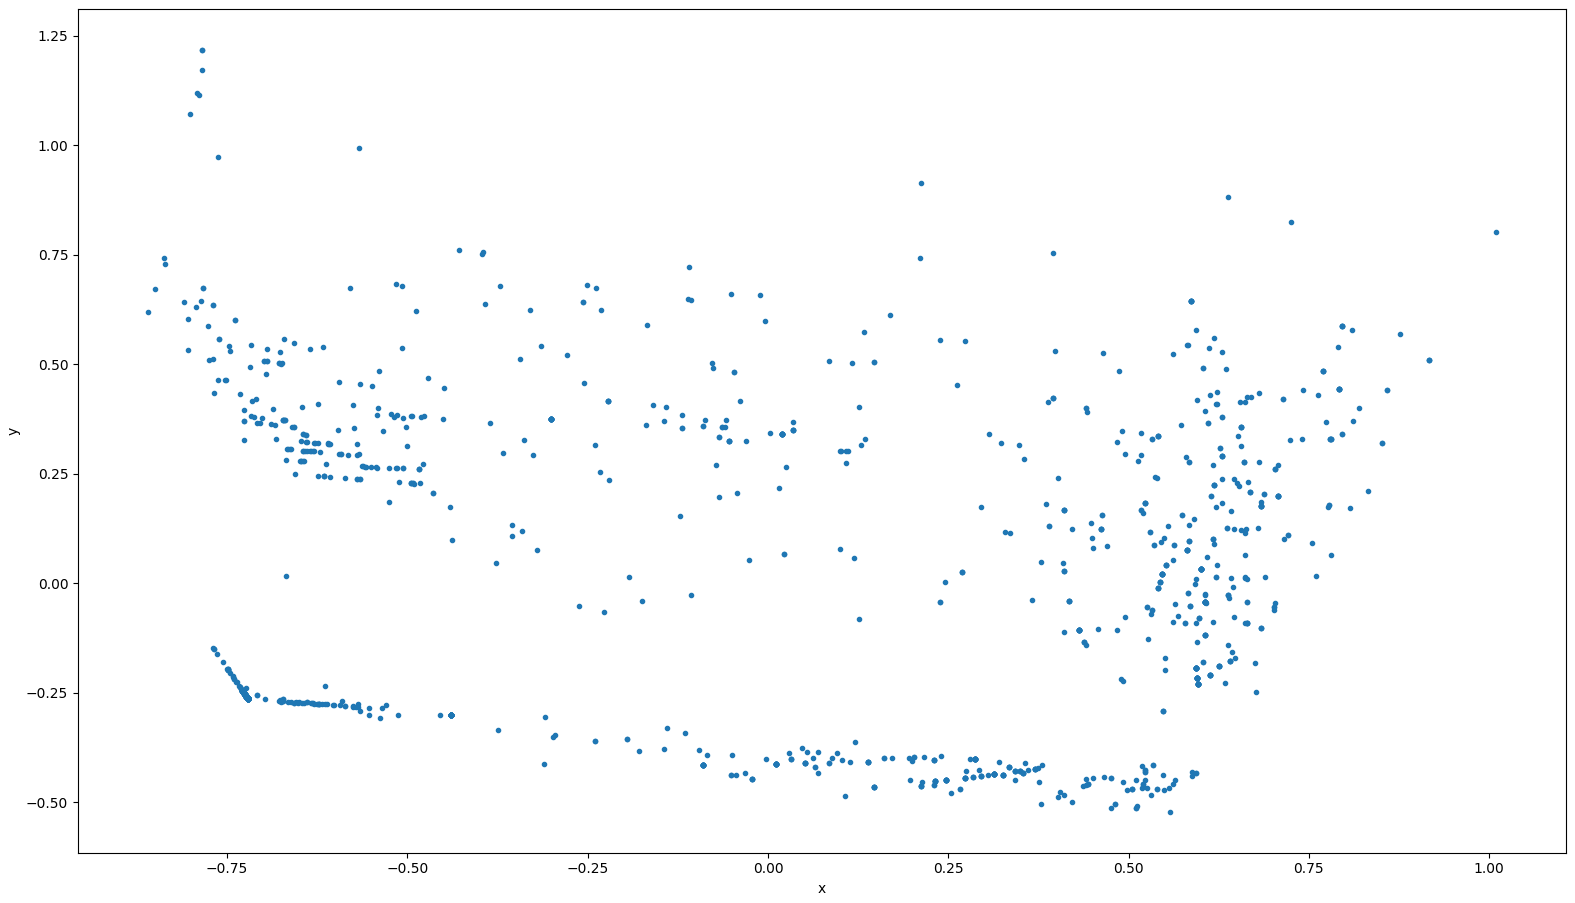
\includegraphics[width=\linewidth]{figs/metrics-pca-13-to-2.png}
	\caption{Visualisation of loop metrics dataset (13-dimensional metric vectors have been projected onto 2d space thanks to PCA algorithm) - blue dots correspond to metric values on single loops.}
	\label{metrics-pca-13-to-2}
\end{figure}

\begin{figure}[h]
	\centering
	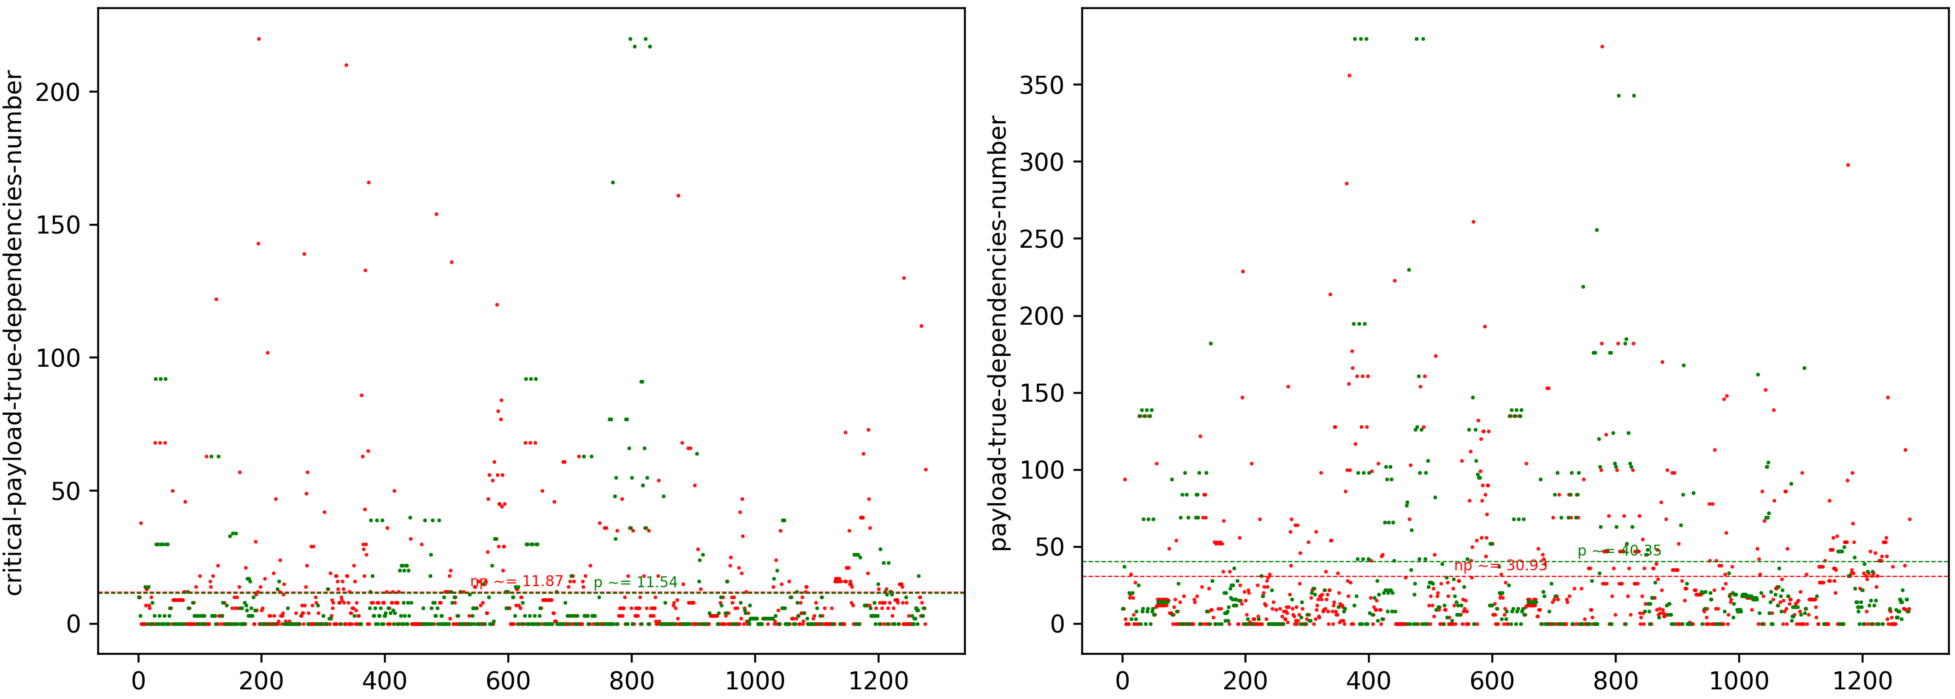
\includegraphics[width=\linewidth]{figs/loop-dependencies-number-1.png}
	\caption{\textit{Critical payload true dependencies number} metric at the top and \textit{payload true dependencies number} metric at the bottom. Red and green dots represent loops, which have not/have been parallelized by ICC compiler correspondingly.}
	\label{loop-dependencies-number-1}
\end{figure}

\begin{figure}[h]
	\centering
	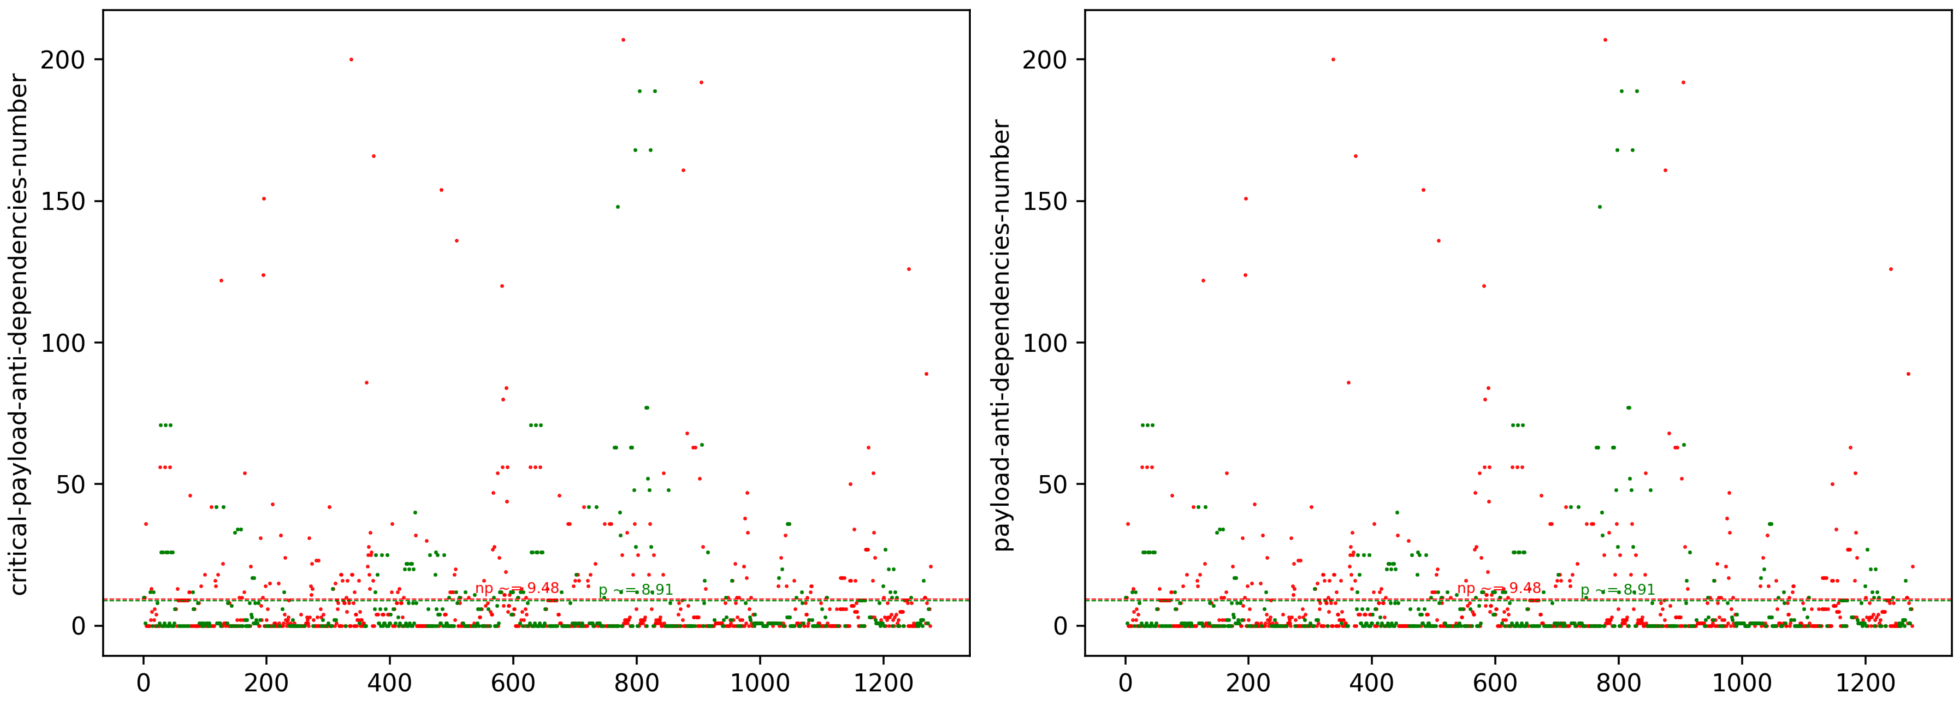
\includegraphics[width=\linewidth]{figs/loop-dependencies-number-2.png}
	\caption{\textit{Critical payload anti dependencies number} metric at the top and \textit{payload anti dependencies number} metric at the bottom. Red and green dots represent loops, which have not/have been parallelized by ICC compiler correspondingly.}
	\label{loop-dependencies-number-2}
\end{figure}

\begin{figure}[htb]
	\centering
	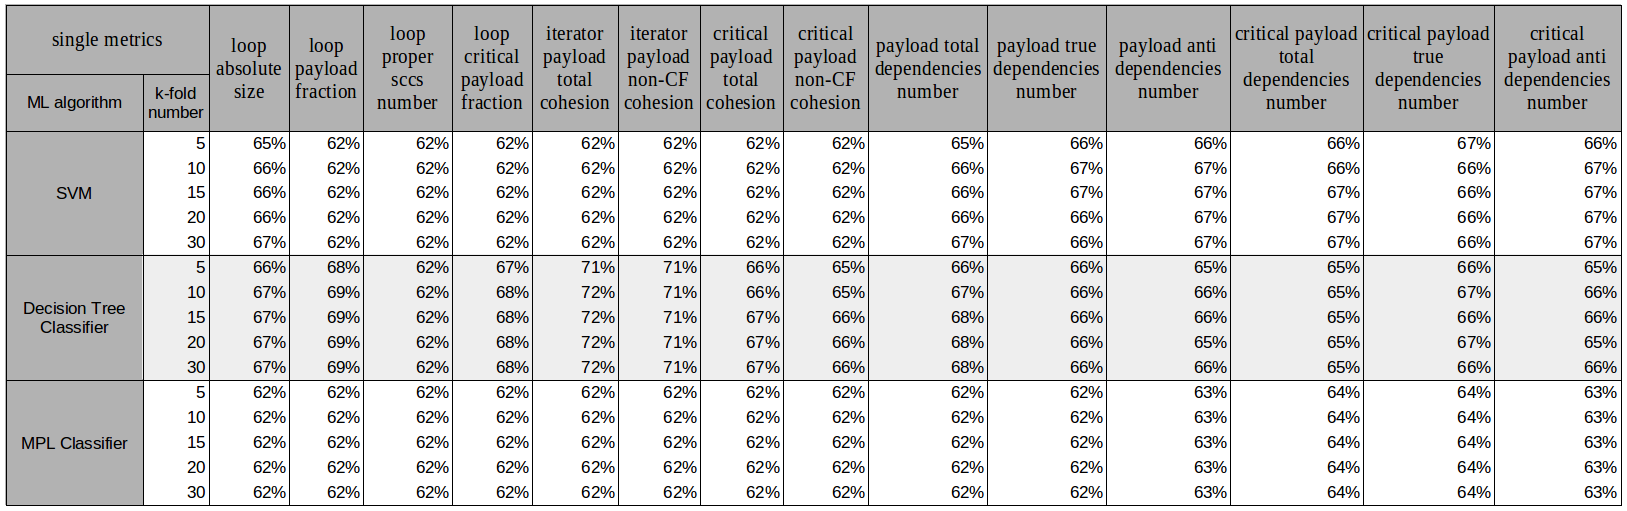
\includegraphics[width=\linewidth]{figs/single-metric-ml-table-1.png}
	\caption{Application of machine learning (ML) techniques (table rows) to different single loop metrics (table columns). Table is populated with average accuracies of these ML methods on the chosen metric for different k-fold cross-validation parameters (5, 10, 15, 20, 30). Every single percentage number has been calculated as the mean of a set of ML classifier runs. }
	\label{single-metric-ml-table-1}
\end{figure}

\begin{figure}[htb]
\centering
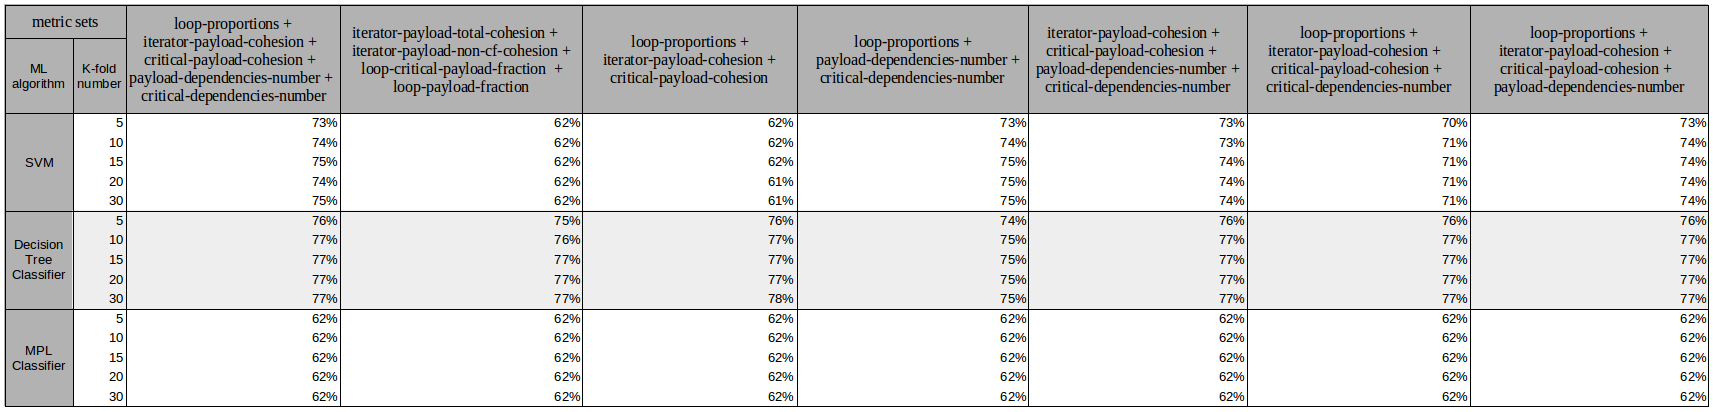
\includegraphics[width=\linewidth]{figs/metric-set-ml-table-1.png}
\caption{Application of machine learning (ML) techniques (table rows) to different single loop metrics (table columns). Table is populated with average accuracies of these ML methods on the chosen metric for different k-fold cross-validation parameters (5, 10, 15, 20, 30). Every single percentage number has been calculated as the mean of a set of ML classifier runs. }
\label{metric-set-ml-table-1}
\end{figure}

\begin{sidewaysfigure}[htb]
\centering
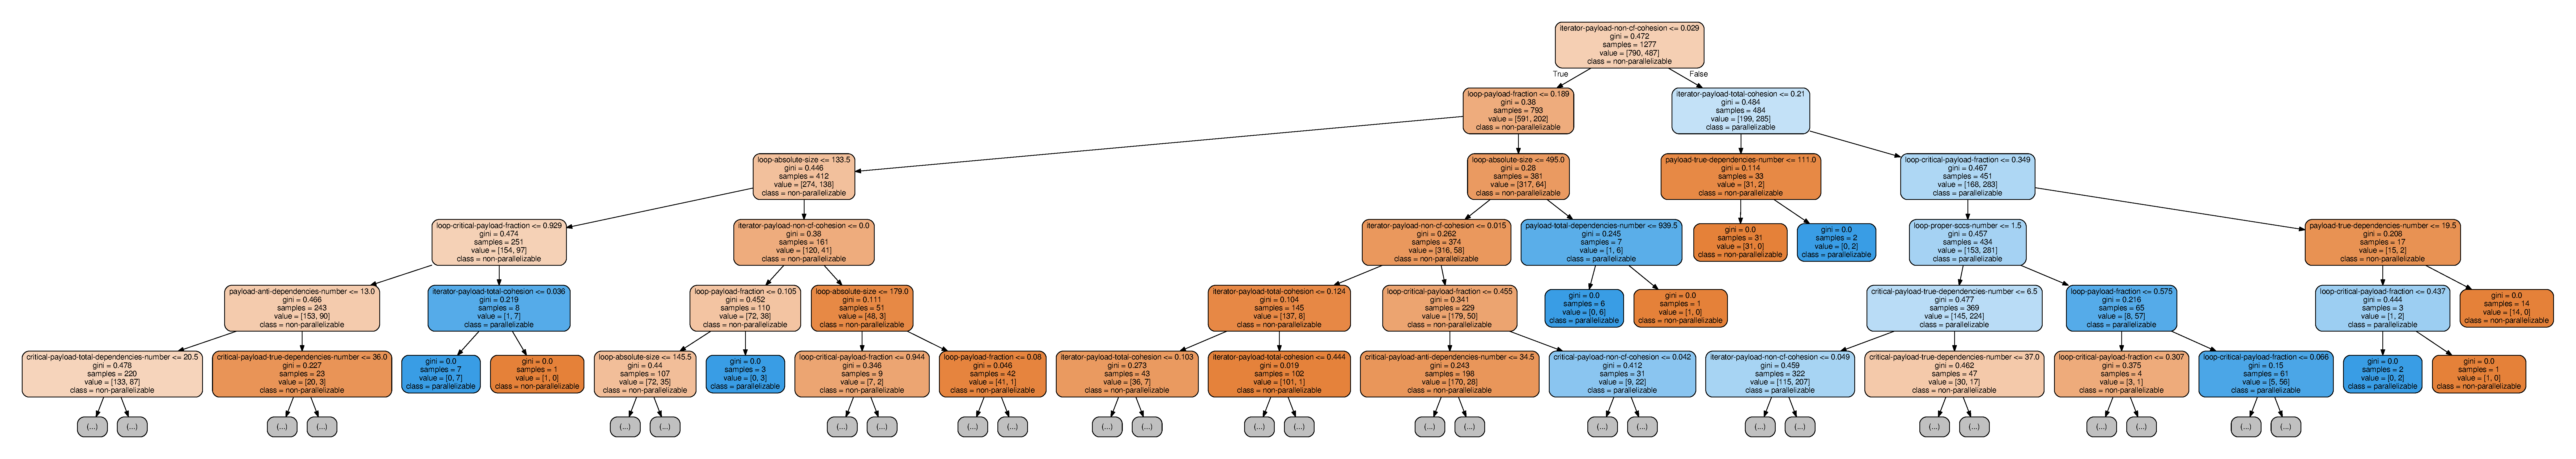
\includegraphics[width=\linewidth]{figs/decision-tree-depth-5.pdf}
\caption{Dataset \ref{analysis-data-table} decision tree, limited to the depth of 5.}
\label{decision-tree-depth-5}
\end{sidewaysfigure}

